\input{settings/settings}  		% Import der Pakete und Stil des Dokuments
\input{settings/adjustments} 	% Weitere Pakete und Anpassungen (Sprache, Quellenverwaltung, etc.)
\input{settings/titlepage}		% Layout der Titelseite

%%%%%%%%%%%%%%%%%%%%%%%%%%%%%%%%%%%%%%%%%%%%%
% Im folgenden Bereich müssen Sie Anpassungen für das Deckblatt der Arbeit vornehmen!
%%%%%%%%%%%%%%%%%%%%%%%%%%%%%%%%%%%%%%%%%%%%%
%
%% Titel und Author 
\titel{Exposé zur Bachelorarbeit: Entwicklung eines Edge-Computing-Systems zur autonomen Schwimmschlammerkennung mittels semantischer Segmentierung auf einem Raspberry Pi in einer Air-Gap-Umgebung}
%\titel{Echtzeit Wasseroberflächenüberwachung und -reinigung eines Nachklärbeckens durch eingebettetes Air Gap System mittels Semantischer Segmentierung und CNN}
\autor{Elias Albrecht}
\matrikelnr{s0589247}
%% Version und Abgabedatum
\version{0.2$\alpha$} 	%ToDo: wird derzeit noch nicht genutzt
\datum{07.04.2022}   	% Abgabedatum der Arbeit
%% Typ der Arbeit
\thesistyp{Bachelorarbeit}
%\thesistyp{Bachelorarbeit}
\abschluss{Bachelor of Engineering (B. Eng.)}
%\abschluss{Bachelor of Engineering (B. Eng.)}
%% Betreuer
\firstExaminer{Prof.~Dr.-Ing. Jochen Kerdels}
\secondExaminer{B. Eng. Christian Rank}
%% Fachbereich
\fachbereich{1 -- Energie und Information --}
\studiengang{Computer Engineering}
%%%%%%%%%%%%%%%%%%%%%%%%%%%%%%%%%%%%%%%%%%%%%
% Ende des Bereichs für Anpassungen
%%%%%%%%%%%%%%%%%%%%%%%%%%%%%%%%%%%%%%%%%%%%%
%% Metadaten zu PDF hinzufügen
\hypersetup{
pdftitle = {\thetitel},
pdfsubject = {\thethesistyp},
pdfauthor = {\theautor},
%pdfkeywords = {Stichwort1, Stichwort2 ...} ,
pdfcreator = {LaTeX with hyperref},
pdfproducer = {pdflatex}
}
%% Pfad zu den Bildern

%% Current Bug-Fixes
% 2024-02 
% Error-Message ! Argument of \MT@gobble@to@nil has an extra }.
% https://tex.stackexchange.com/questions/702778/argument-of-mtgobbletonil-has-an-extra
\microtypesetup{nopatch=item}


\usepackage{csquotes}
\usepackage{graphicx} % Required for inserting images
\usepackage[ngerman]{babel}

\usepackage{array}
\usepackage{tabularx}
\usepackage[table,xcdraw]{xcolor}
\usepackage{colortbl}
\usepackage{subfigure}


\addbibresource{bibliography.bib}



\begin{document}

\maketitle

\section{Problemstellung}



In Klärwerken werden Belebungslinien eingesetzt, die das Bakterienwachstum fördern sollen, um die Verarbeitung des Klärwassers voranzutreiben. Am Ende dieser biologischen Prozesse wird das Wasser in Nachklärbecken weitergeleitet, die dieses in 4 Zonen unterteilt: Klarwasser-, Trenn-, Speicher- und Räum-/Eindickzone. Mittels sogennanter Räumer wird das Wasser gleichmäßig verteilt und der gram-positive Schlamm am Beckengrund in der Eindickzone abgeführt. Darüber befinden sich Speicher- und Trennzone, in denen sich die Partikel absetzen oder wie im Fall der gram-negativen Fadenorganismen auf der Klarwasserzone anreichern, wo sie Klär-/Blähschlamm bilden. Diese Art Schlamm wird ebenfalls gereinigt, da das übermäßige Wachstum zu einer Verdickung der Schicht führt. Das kann bewirken, dass der Ablauf des Klarwassers verschmutzt wird, weil sich die Schichten vermischen. Hierdurch entstehen weitere Probleme in der Klärung des Wassers, da die Qualitätsansprüche für (beispielsweise) eine Flockungsfiltration nicht erfüllt werden. \\ \\

SSR: Schwimmende-Schwimmschlamm-Räumer werden eingesetzt um über eine oder mehrere Förderschnecken den Oberflächenbelag an einem Schwimm-
schlamm-Schlürftrichter zu konzentrieren. Der Inhalt wird abgefördert, um die Oberfläche sauber zu halten, damit der Anteil an entsprechenden Fadenbakterien nicht überhand nimmt und das Gleichgewicht des Beckens stört.
Die bisherige Steuerung funktioniert über einen Timer, der zwischen Winter- und Sommerbetrieb umgeschalten wird, um auf die Veränderungen des Bakterienwachstums und der damit einhergehenden Oberflächen-
beschaffenheit annäherungsweise einzugehen. Da die biologischen Begebenheiten hierbei deutlich komplexer als ein simpler Zeitintervall sind, ergibt sich ein Optimierungsgedanke.


\begin{figure}[hb!]
    \centering
    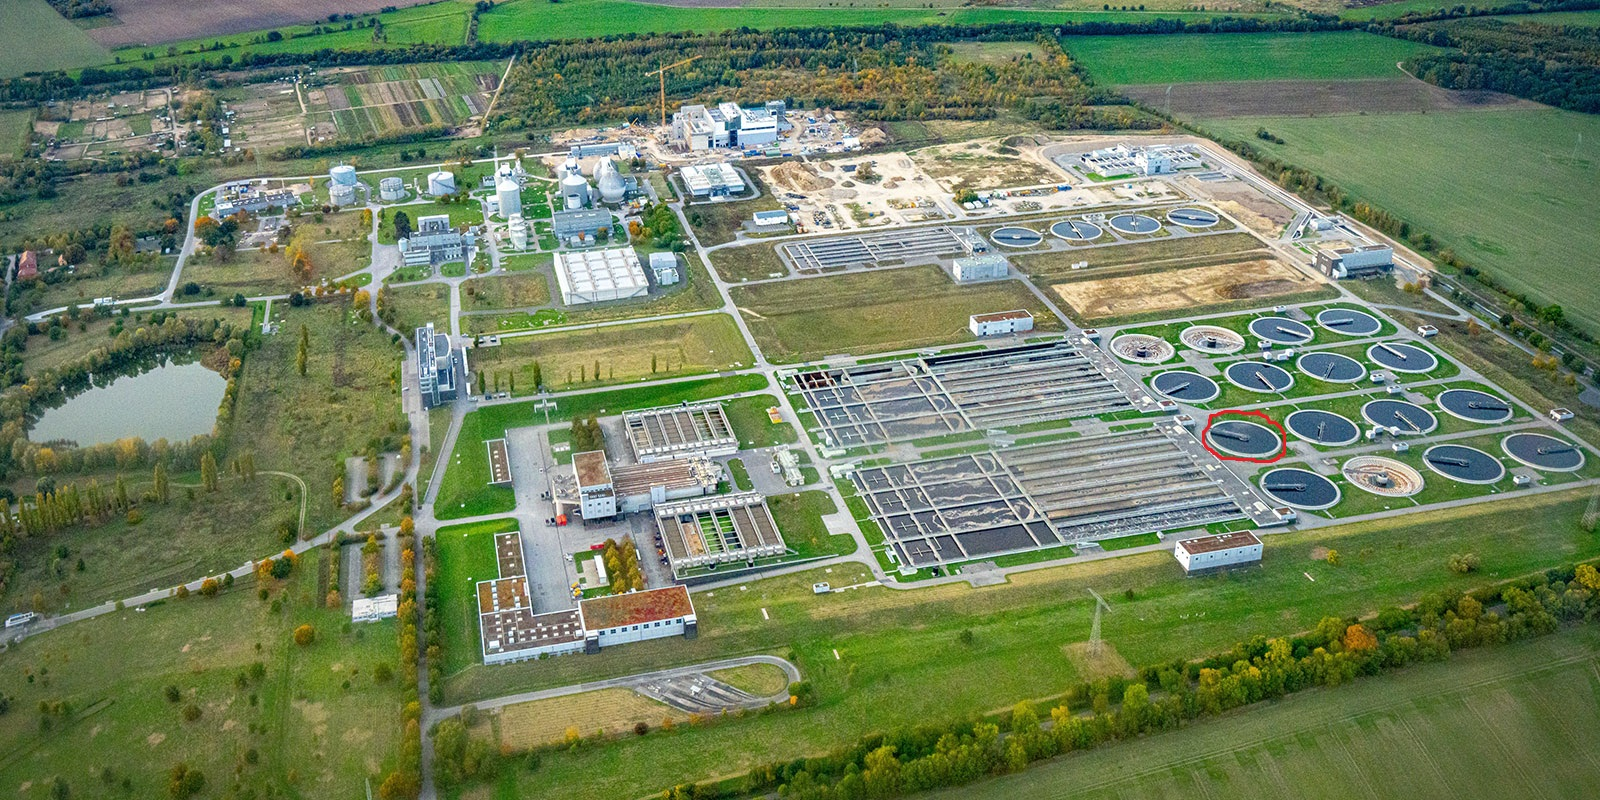
\includegraphics[width=1\linewidth]{pictures/Klärwerk Waßmannsdorf.jpg}
    \caption{Gelände des Klärwerks Waßmannsdorf}
    \label{fig:was}
\end{figure}




\section{Forschungstand}

Innerhalb der Convolutional Neural Networks (CNN) existieren bereits erfolgreiche Architekturen für semantische Segmentierung wie das U-Net. Diese wurden für leistungsschwachere Hardware in Form des MobileNet oder EfficientNet optimiert, um die benötigte Rechenlast zu reduzieren. \\ \\

Auch die optische Analyse von Schwimmschlamm findet im Labormaßstab bereits statt, aber stabile Implementierungen für den autarken Realbetrieb unter Air-Gap-Bedingungen werden bislang kaum angewendet.  


\section{Erkenntnisinteresse}

Die Arbeit bietet umfassende Möglichkeiten zur Auseinandersetzung mit dem interdisziplinären Aufbau der Abwasserklärung und Einblicke in machinelles Lernen mit einem Fokus auf Semantische Segmentierung sowie die Arbeit in isolierten Linux-Umgebungen und Raspberry PI Programmierung.
\\ \\
Auf Software-Ebene soll eine Bildverarbeitungspipeline realisiert werden, die Bilder mit dem Raspberry aufnimmt und für das Neuronale Training aufbereitet. Sämtliche Anforderungen unterliegen einem hohen Maß an Stabilität und Resilienz gegenüber Umwelteinflüssen. 

\begin{figure}[t!]
    \centering
    \subfigure[]{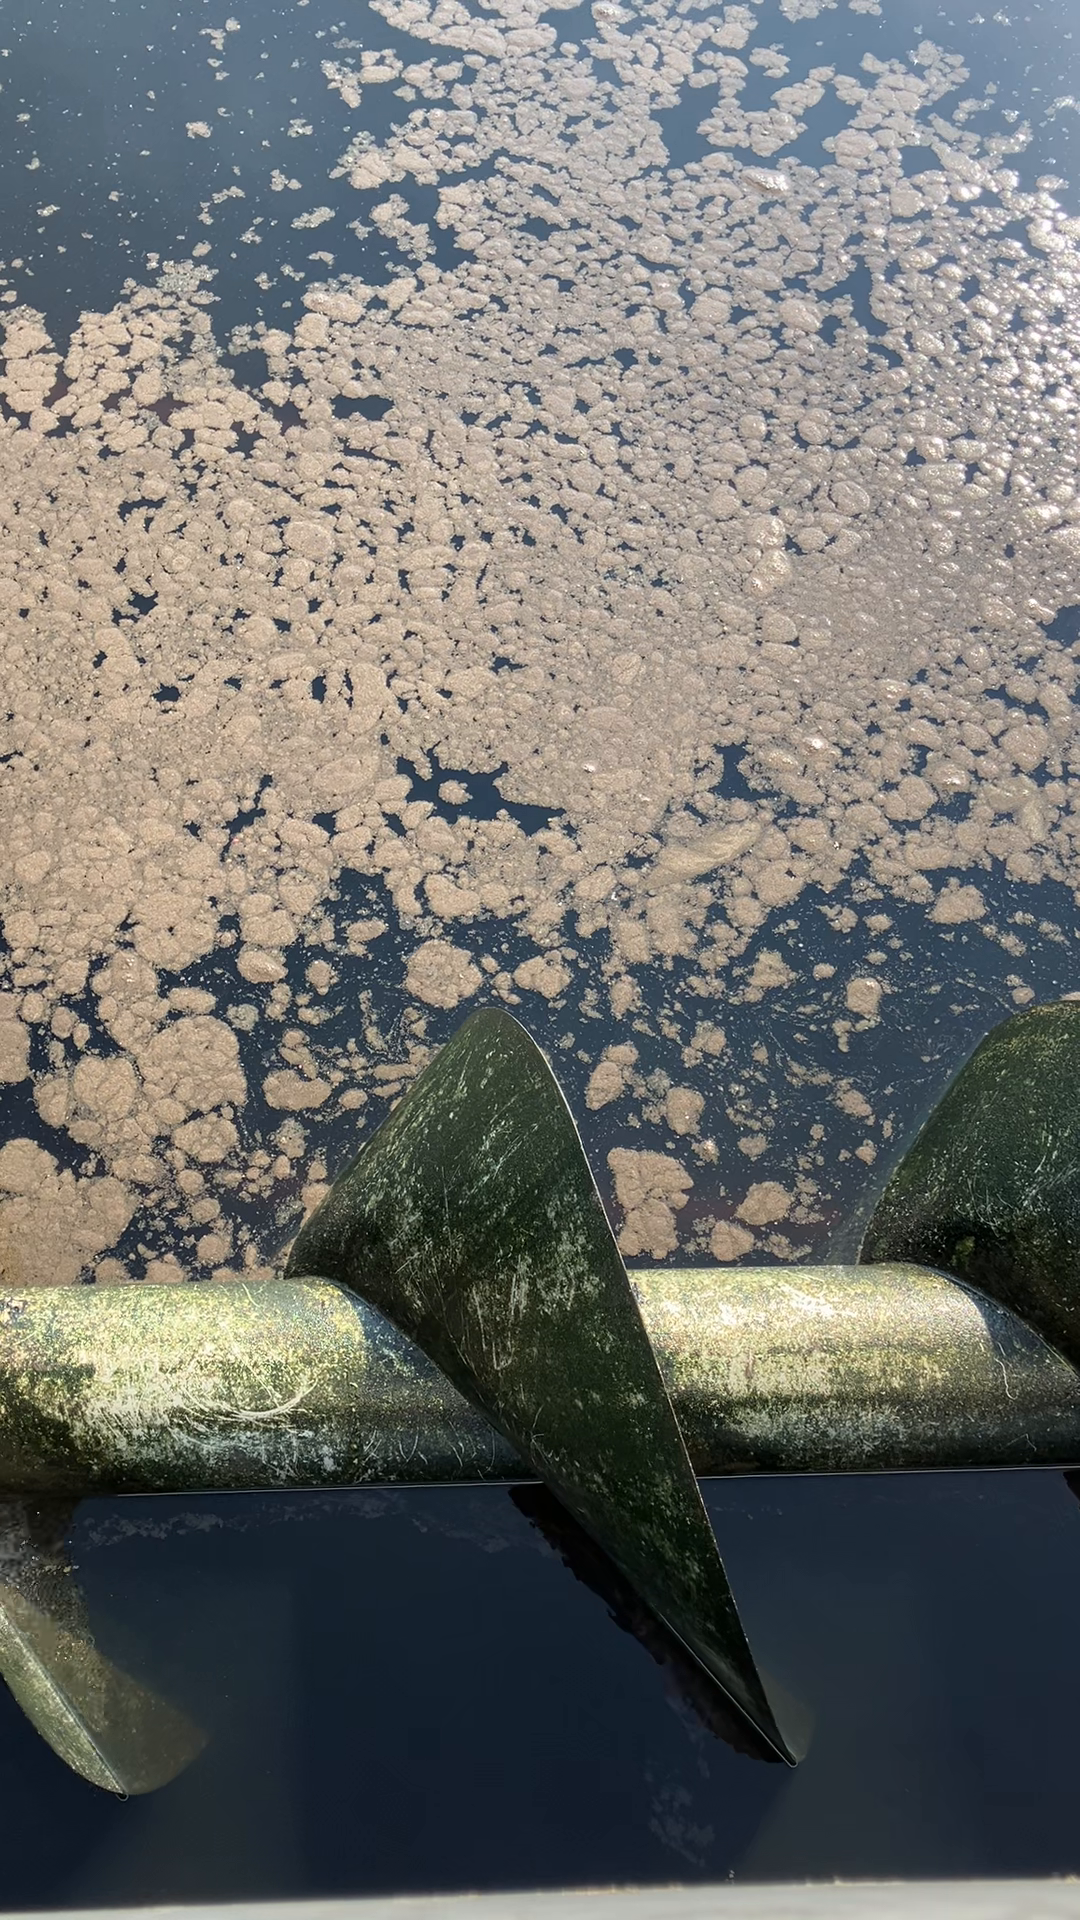
\includegraphics[width=0.49\linewidth]{pictures/img_0001.png}}
    \subfigure[]{
\includegraphics[width=0.49\linewidth]{pictures/0001_final.png}}
    
    
    \caption{Vergleich Wasseroberfläche Original vs. Bitmaske}
    \label{fig:oberfläche}
\end{figure}


\section{Fragestellung}

Wie lässt sich der Energieverbrauch und die Prozessstabilität einer Timer-gesteuerten Schwimmschlammklärung durch eine bedarfsorientierte Lösung optimieren? 

\section{Hypothese}

Anhand der empirischen Messdaten zur Oberflächenreinigung im Ist-Zustand in Waßmannsdorf lässt sich ableiten, dass eine Optimierung in Bezug auf Energieverbrauch und Wasserqualität des zugrunde liegenden Systems im signifikanten Maßstab möglich ist. 

\section{Methode \& Material}
Die Arbeit nutzt einen quantitativen Ansatz:
\begin{itemize}
    \item \textbf{Datenakquise:} Nutzung von Bildmaterial aus der Anlage Waßmannsdorf.
    \item \textbf{Preprocessing:} Implementierung einer semi-automatisierten Annotations-Pipeline mittels HSV-Farbraumtransformation in OpenCV, um den manuellen Labeling-Aufwand zu reduzieren.
    \item \textbf{Modellierung:} Training und Quantisierung eines MobileNet-V2 Modells.
    \item \textbf{Hardware:} Implementierung auf einem Raspberry Pi 5 in einer isolierten Linux-Umgebung (Air-Gap).
\end{itemize}

\section{Vorläufige Gliederung}
\begin{enumerate}
    \item Einleitung (Problemstellung, Zielsetzung)
    \item Theoretische Grundlagen
        \subitem 2.1 Verfahrenstechnik der Nachklärung und Schwimmschlamm
        problematik
        \subitem 2.2 Deep Learning zur semantischen Segmentierung
        \subitem 2.3 Edge-Computing und IT-Sicherheit (Air-Gap)
    \item Methodik und Implementierung
        \subitem 3.1 Datensatzgenerierung und semi-automatisches Labeling
        \subitem 3.2 Modell-Training und Optimierung für Edge-Hardware
        \subitem 3.3 Hardwareaufbau und GPIO-Aktorik
    \item Evaluation und Ergebnisse
        \subitem 4.1 Genauigkeitsanalyse (IoU-Metriken)
        \subitem 4.2 Vergleich der Steuerungsstrategien (Timer vs. Bedarfsorientiert)
    \item Fazit und Ausblick
    \item Verzeichnisse
\end{enumerate}

%\newpage

\section{Zeitplan}

\begin{center}
    


\begin{tabular}{|l|l|l|l|l|l|l|l|l|l|l|}
\hline
\rowcolor[HTML]{DAE8FC} 
\textbf{Woche}                                             & 1                        & 2                        & 3                        & 4                        & 5                        & 6                        & 7                        & 8                        & 9                        & 10                       \\ \hline
\cellcolor[HTML]{9B9B9B}\textbf{Fundament und Setup}       & \cellcolor[HTML]{9B9B9B} & \cellcolor[HTML]{9B9B9B} & \cellcolor[HTML]{9B9B9B} & \cellcolor[HTML]{FFFFFF} & \cellcolor[HTML]{FFFFFF} &                          &                          &                          &                          &                          \\ \hline
Finalisierung der Literaturrecherche                       & \cellcolor[HTML]{C0C0C0} &                          &                          &                          &                          & \cellcolor[HTML]{FFFFFF} &                          &                          &                          &                          \\ \hline
Anforderungsanalyse \& Systemspezifikation                 &                          & \cellcolor[HTML]{C0C0C0} &                          &                          &                          &                          &                          &                          &                          &                          \\ \hline
Explorative Datenanalyse                                   &                          &                          & \cellcolor[HTML]{C0C0C0} &                          &                          &                          &                          &                          &                          &                          \\ \hline
\cellcolor[HTML]{9B9B9B}\textbf{Kernarbeit \& Optimierung} &                          &                          &                          & \cellcolor[HTML]{9B9B9B} & \cellcolor[HTML]{9B9B9B} & \cellcolor[HTML]{9B9B9B} &  &                          &                          &                          \\ \hline
Modell-Iteration \& Parameter-Tuning                       &                        &                          &                          & \cellcolor[HTML]{C0C0C0} &  &                          &                          &                          &                          &                          \\ \hline
Validierung der Farb-Segmentierung  &   &   &    &    &  \cellcolor[HTML]{C0C0C0} &  &  &                          &                          &                          \\ \hline
Hardware-Integration &  &  &  &  &  & \cellcolor[HTML]{C0C0C0} &  &  &  &                          \\ \hline
\cellcolor[HTML]{9B9B9B}\textbf{Fundament und Setup} &   &   &  &  &  &  &    \cellcolor[HTML]{9B9B9B}   & \cellcolor[HTML]{9B9B9B} & \cellcolor[HTML]{9B9B9B} & \cellcolor[HTML]{9B9B9B} \\ \hline
Systemtest im Realbetrieb &  &  &  &  &  &  & \cellcolor[HTML]{C0C0C0} & \cellcolor[HTML]{C0C0C0} &  &  \\ \hline
Intensivschreibphase  &  &   &  &    &   &    &  \cellcolor[HTML]{C0C0C0}  & \cellcolor[HTML]{C0C0C0} &   &     \\ \hline
Review &  &  &   &                          &                          &                          &                          & \cellcolor[HTML]{FFFFFF} & \cellcolor[HTML]{C0C0C0} &                          \\ \hline
Puffer \& Abgabe                                           &                          &                          &                          &                          &                          &                          &                          &                          &                          & \cellcolor[HTML]{C0C0C0} \\ \hline
                                             
\end{tabular}


\end{center}


\section{Eigene Vorarbeit}

Im Rahmen des Studienpraktikums wurde das Thema untersucht. Die Grundlagen für die Funktionsweise eine Klärwerks wurden in Form von Führungen, Rückfragen und eigener Recherche kennengelernt, um eine Basis an Wissen bilden zu können. Darüber hinaus wurden Ansprüche an das Projekt formuliert, Hard- und Software recherchiert und organisiert sowie Arbeitsprozesse geplant. Insbesondere die Einrichtung einer funktionierenden Umgebung unterlag besonderen Anforderungen. So wurde ein Dell Pro Rugged 14 Laptop im Air Gap mit Linux Mint sowie der notwendigen Software inklusive Abhängigkeiten ausgestattet, um der kritischen Infrastruktur gerecht zu werden. Hiermit wurden auch die Grundsteine für die Programmierung des Raspberry PI 5 gelegt. 











  

\end{document}
